\documentclass[12pt]{article}
\usepackage{graphicx}%Package um Grafiken einzufügen
\graphicspath{ {assets/} }
\usepackage[ngerman]{babel}%Sprache Deutsch einstellen
\usepackage[headheight=15pt, a4paper, left=40mm, top=20mm, bottom=20mm, right=20mm]{geometry}
%\usepackage[]{fontspec}
%\setmainfont{Inter.ttf}
\usepackage[]{fancyhdr}
\pagestyle{fancy}
%\setlength{\headheight}{16pt}
\lhead{\leftmark}
\rhead{Phillip Bronzel} 

\usepackage[style=authoryear, backend=biber]{biblatex}
\addbibresource{references.bib}
\usepackage{csquotes}

\usepackage{eso-pic}
\newcommand\BackgroundPic{
    \put(0,0){
    \parbox[b][\paperheight]{\paperwidth}{%
    \vfill
    \centering
    
\includegraphics[width=\paperwidth,height=\paperheight]{assets/titlebackground.pdf}
    \vfill
    }}}

\usepackage{chronology}

\title{Machine Learning in Smartphone Apps}
\date{Phillip Bronzel \today}
\author{ASGSG Informatik, 2020/2021}

\begin{document}
  \AddToShipoutPicture*{\BackgroundPic}
  \maketitle
  \pagenumbering{gobble}
  \begin{center}
   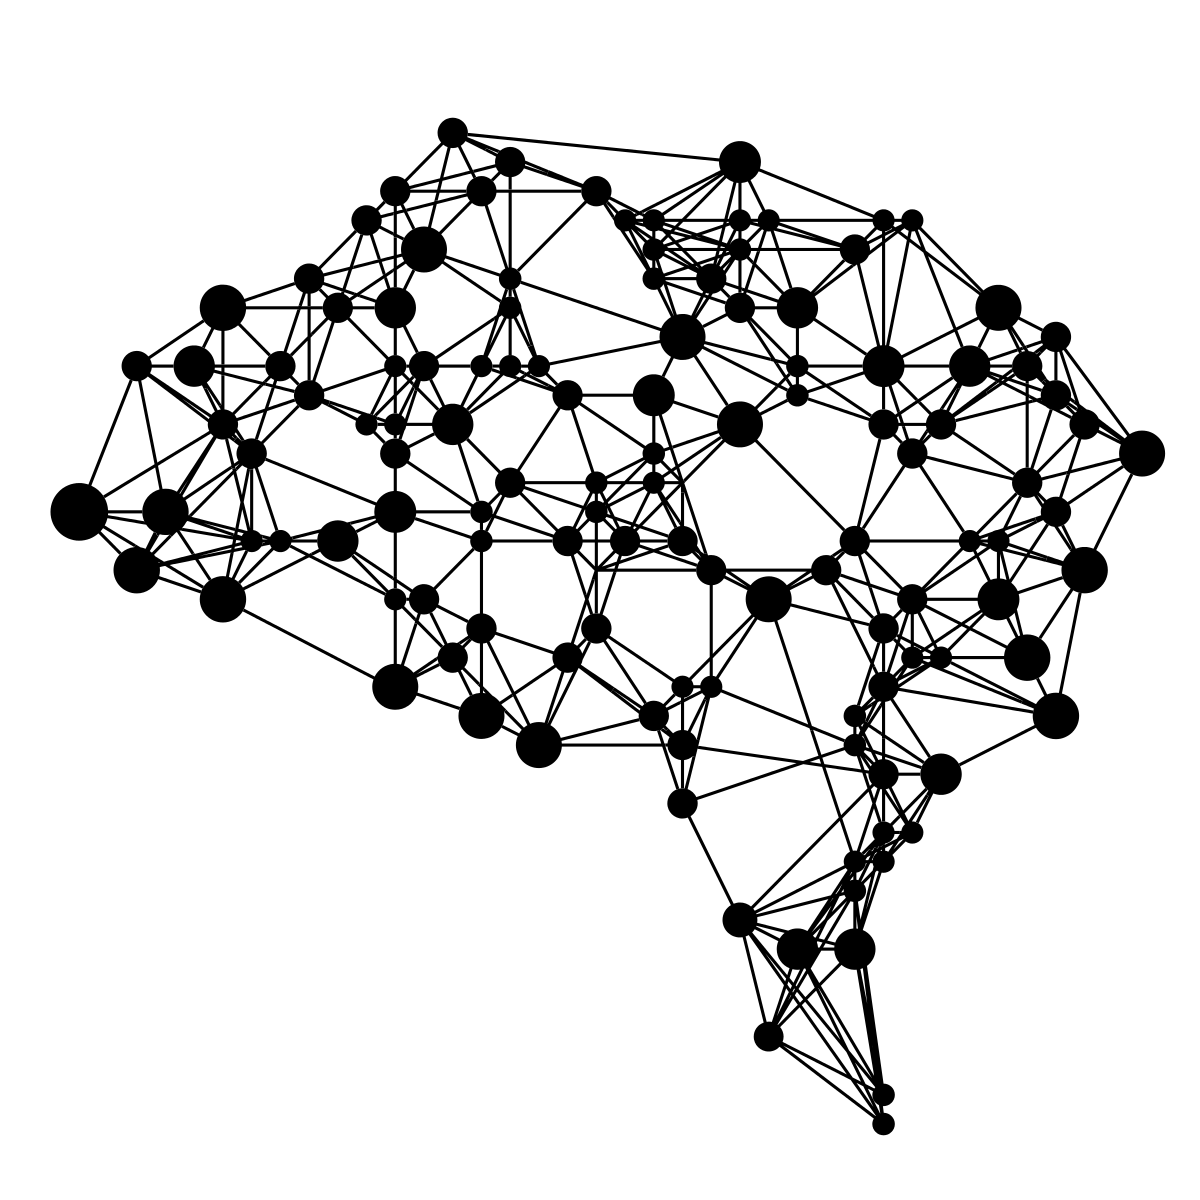
\includegraphics[totalheight=10cm]{titlepage.png}
   \cite{titlepageimage}
  \end{center}

  \newpage
  \vspace*{\fill}
  \input{lib/erklärung.tex}
  \vspace*{\fill}

  \newpage
  \pagenumbering{arabic}
  \tableofcontents

  \newpage
  \input{lib/einführung.tex}%TODO: Kapitel der App einfügen

  \newpage
  \section{Herkömmliche neuronale Netzwerke}

\subsection{Geschichte}

Schon ab 1940 versuchten Forscher den Aufbau eines menschlichen Gehirns mit elektronischen Schaltkreisen nachzubauen. Man versuche also die die einzelnen Neuronen samt Verbindungen zu imitieren. Immer wieder gab es kleine Durchbrüche, wie zum Beispiel im Jahr 

\subsubsection{Zeitstrahl}

\begin{chronology}[10]{1940}{2020}{\textwidth}
    \event[1940]{1948}{Erste Forschungen}
    \event[1985]{1986}{two}
    \event{\decimaldate{25}{12}{2001}}{three}
\end{chronology}
    

\subsection{Aufbau}

  \newpage
  \printbibliography[heading=bibintoc, title={Literaturverzeichnis}]
\end{document}